% Couverture Thèse TPT Latex v2
% Fabrice Linot 04/12/11

\documentclass[11pt,a4paper]{book}
\usepackage[left=1.3cm,top=0cm,right=1.3cm,bottom=1.2cm]{geometry}
\usepackage{graphicx}
\usepackage{eso-pic}
\usepackage{array}
\usepackage[french]{babel}
\usepackage[utf8x]{inputenc}
\usepackage[T1]{fontenc}
\usepackage{textcomp}
\usepackage{helvet}	% or \usepackage{lmodern}
\renewcommand\textnumero{n$^{\textsf{{\tiny O}}}$}
\renewcommand{\familydefault}{\sfdefault}

\usepackage{ifpdf}
\newcommand\BackgroundPic{
\ifpdf
	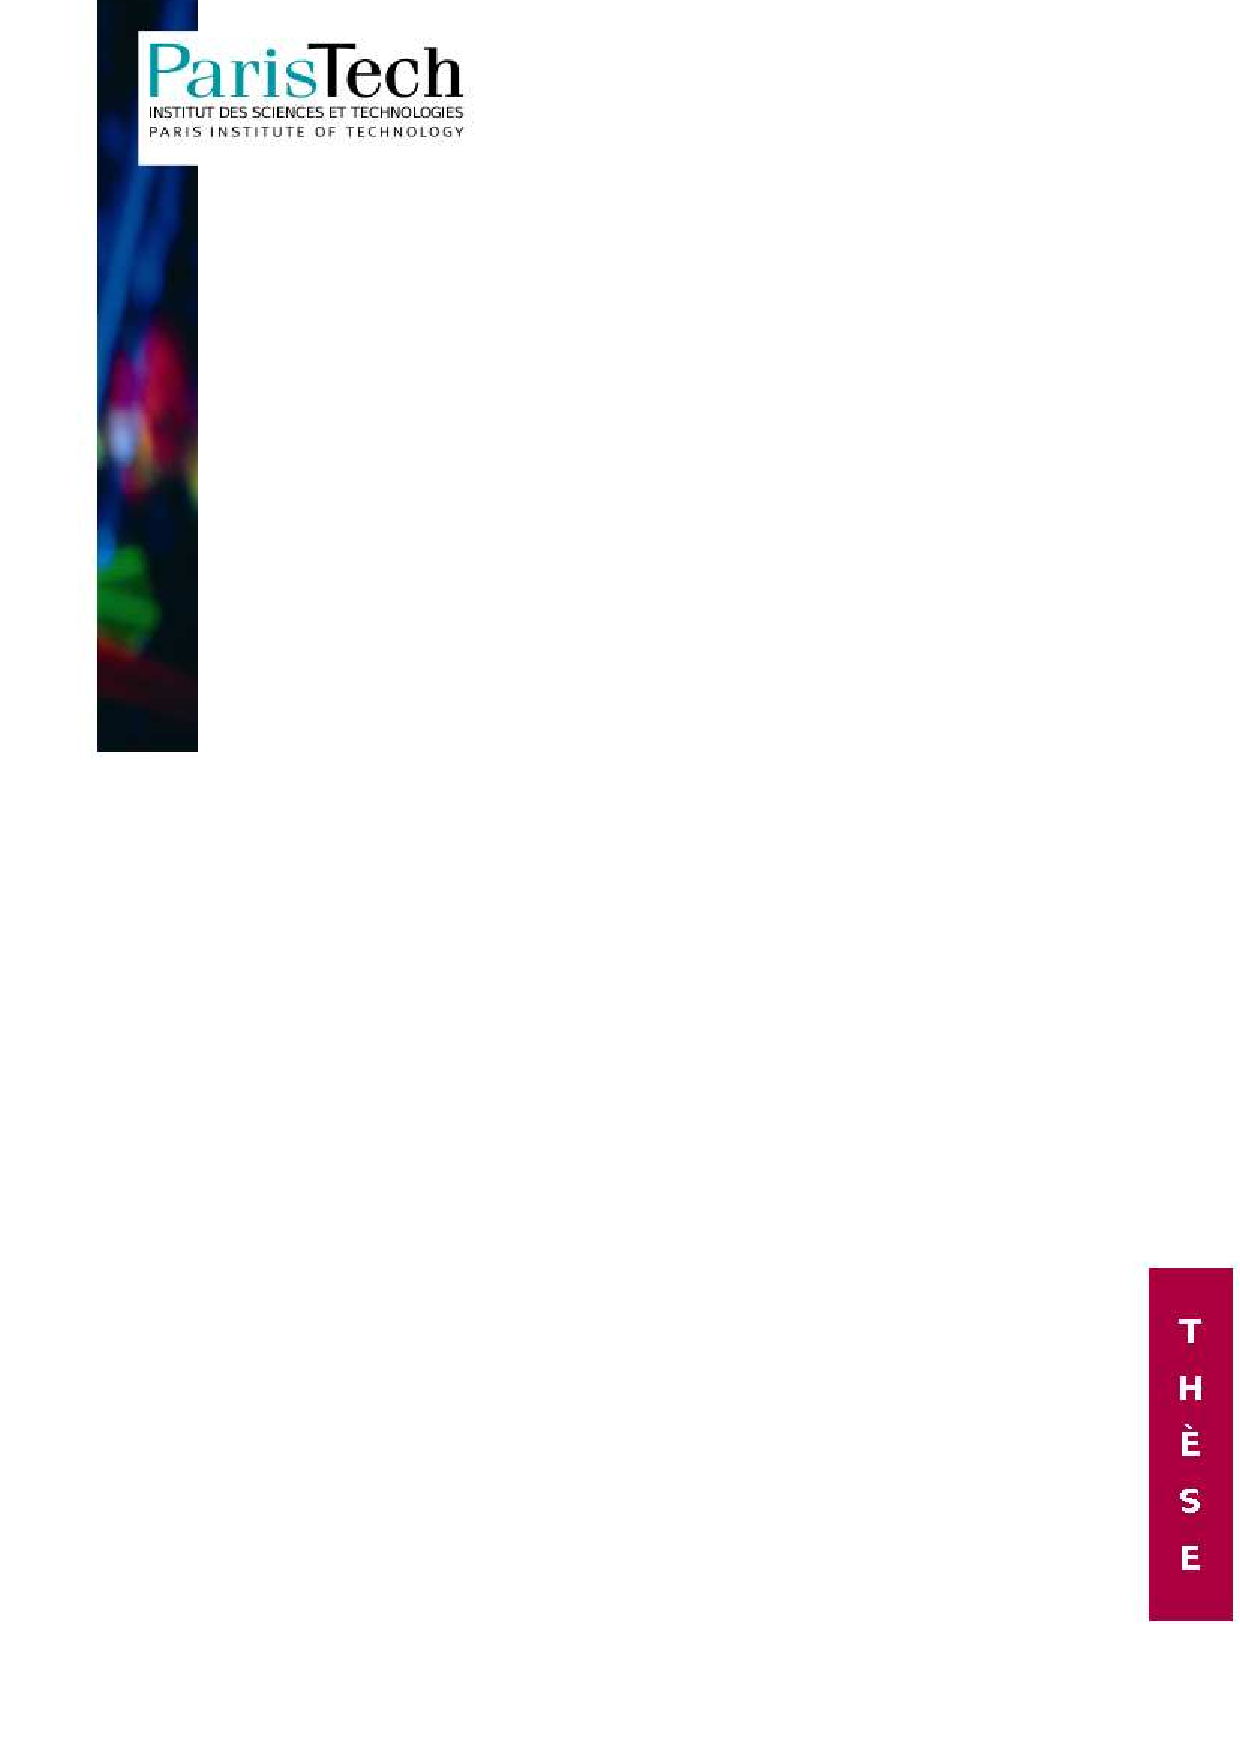
\includegraphics[height=\paperheight,width=\paperwidth]{BackgroundTPT_Premiere.pdf}
\else
	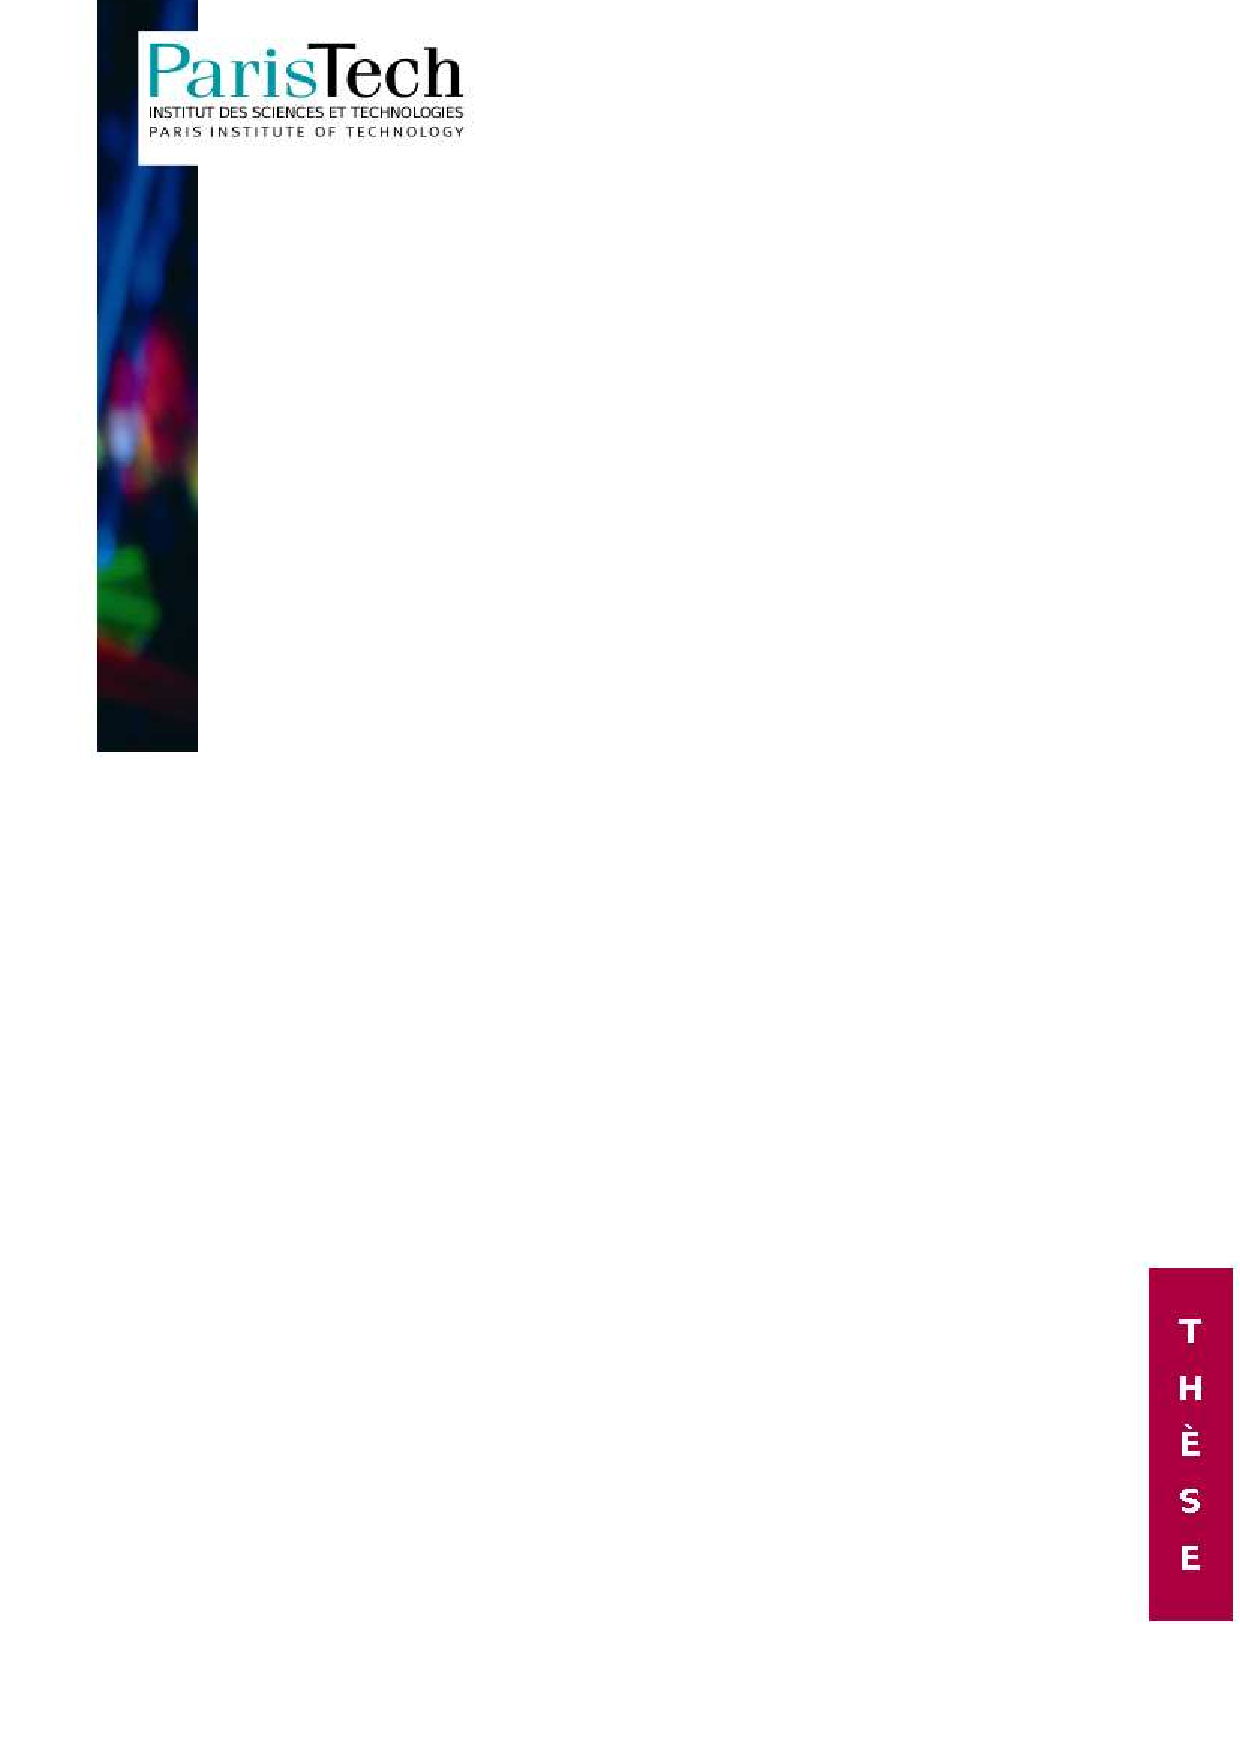
\includegraphics[height=\paperheight,width=\paperwidth]{BackgroundTPT_Premiere.pdf}
\fi
}

\pagestyle{empty}

\begin{document}
\AddToShipoutPicture*{\BackgroundPic}
~


\begin{flushright}


\includegraphics[scale=0.45]{logo_TPT.pdf}

{\small {2015-ENST-0083~~~~}}
\end{flushright}



%\vspace{0.cm}
\begin{center}
%



\includegraphics[scale=0.65]{logo_edite.pdf} \\
{\small {EDITE - ED 130}}


%
\vspace{.5cm}
%
%
%
%{\Large École doctorale \textnumero XX: texte}\\		% version une ligne
%{\Large École doctorale \textnumero XX:\\ texte}\\		% version deux lignes (changer les espaces en conséquence
%
%
%
\vspace{1.0cm}
%
%
%
{\LARGE {\bf Doctorat ParisTech}}\\
\vspace{1.1cm}
{\LARGE {\bf T H È S E}}\\
\vspace{0.5cm}
{\normalsize {\bf pour obtenir le grade de docteur délivré par}}\\
%
%
%
\vspace{.9cm}
%
%
%
%
{\LARGE {\bf TELECOM ParisTech}}\\
\vspace{0.6cm}
{\Large {\bf Spécialité \og Computer Science and Multimedia \fg}}\\
%
%
%
\vspace{.8cm}
%
%
%
{\normalsize {\it présentée et soutenue publiquement par}}\\
\vspace{0.7cm}
{\Large {\bf Ahmad ASSAF}}\\
\vspace{0.24cm}
{\normalsize 18 12 2015}\\
%
%
%
\vfill
%
%
%
\textcolor[RGB]{191,18,56}{
\noindent
{\LARGE {\bf Enabling Self-Service Data Provisioning\\[.6cm]Through Semantic Enrichment of Data}}\\
}
%
%
%
\vfill~\vfill
%
%
%
{\normalsize
\begin{tabular}{c}
Directeur de thèse:					{\bf Dr.\ Rapha\"el TRONCY}\\
Co-encadrement de la thèse:		{\bf Dr.\ Aline SENART}
\end{tabular}
}
\end{center}
%
%
%
\vfill
%
%
%
\flushleft
\begin{minipage}{.9\textwidth}	% ou .91\textwidth si vous n'avez pas assez de place
{\bf Jury}\\
% Mme/M. Prénom NOM, Titre, Unité de recherche, Ecole
{\bf Philippe CUDR\'{E}-MAUROUX}, {\small Prof, University of Fribourg, Switzerland}\\
{\bf Marie Aude AUFAURE}, {\small Prof,  \'{E}cole Centrale Paris, France}\\
{\bf Pierre SENELLART}, {\small Prof, Telecom ParisTech, France}\\
{\bf Stefan DIETZE}, {\small Dr, Leibniz University, Germany}\\

\end{minipage}\\
%
%
%
\vspace{-.3cm}
%
%
%
\centering
{\bf TELECOM ParisTech}\\
{\small école de l'Institut Télécom - membre de ParisTech}
%
%
%
\end{document}
